\documentclass[10pt,oneside]{memoir}
\usepackage{layouts}[2001/04/29]
\makeglossary
\makeindex

\def\mychapterstyle{default}
\def\mypagestyle{headings}
\def\revision{}

%%% need more space for ToC page numbers
\setpnumwidth{2.55em}
\setrmarg{3.55em}

%%% need more space for ToC section numbers
\cftsetindents{part}{0em}{3em}
\cftsetindents{chapter}{0em}{3em}
\cftsetindents{section}{3em}{3em}
\cftsetindents{subsection}{4.5em}{3.9em}
\cftsetindents{subsubsection}{8.4em}{4.8em}
\cftsetindents{paragraph}{10.7em}{5.7em}
\cftsetindents{subparagraph}{12.7em}{6.7em}

%%% need more space for LoF numbers
\cftsetindents{figure}{0em}{3.0em}

%%% and do the same for the LoT
\cftsetindents{table}{0em}{3.0em}

%%% set up the page layout
\settrimmedsize{\stockheight}{\stockwidth}{*}	% Use entire page
\settrims{0pt}{0pt}

\setlrmarginsandblock{1.5in}{1.5in}{*}
\setulmarginsandblock{1.5in}{1.5in}{*}

\setmarginnotes{17pt}{51pt}{\onelineskip}
\setheadfoot{\onelineskip}{2\onelineskip}
\setheaderspaces{*}{2\onelineskip}{*}
\checkandfixthelayout

\usepackage{fancyvrb}			% Allow \verbatim et al. in footnotes
\usepackage{graphicx}			% To include graphics in pdf's (jpg, gif, png, etc)
\usepackage{booktabs}			% Better tables
\usepackage{tabulary}			% Support longer table cells
\usepackage[utf8]{inputenc}		% For UTF-8 support
\usepackage[T1]{fontenc}		% Use T1 font encoding for accented characters
\usepackage{xcolor}				% Allow for color (annotations)

%\geometry{landscape}			% Activate for rotated page geometry

%\usepackage[parfill]{parskip}	% Activate to begin paragraphs with an empty
								% line rather than an indent


\def\myauthor{Author}			% In case these were not included in metadata
\def\mytitle{Title}
\def\mykeywords{}
\def\mybibliostyle{plain}
\def\bibliocommand{}

\VerbatimFootnotes
\def\myauthor{Jenee Hughes}
\def\baseheaderlevel{1}
\def\format{complete}
\def\mytitle{ThesisDocumentsMelodyMatcher}


%
%	PDF Stuff
%

%\ifpdf							% Removed for XeLaTeX compatibility
%  \pdfoutput=1					% Removed for XeLaTeX compatibility
  \usepackage[
  	plainpages=false,
  	pdfpagelabels,
  	pdftitle={\mytitle},
  	pagebackref,
  	pdfauthor={\myauthor},
  	pdfkeywords={\mykeywords}
  	]{hyperref}
  \usepackage{memhfixc}
%\fi							% Removed for XeLaTeX compatibility


%
% Title Information
%


\ifx\latexauthor\undefined
\else
	\def\myauthor{\latexauthor}
\fi

\ifx\subtitle\undefined
\else
	\addtodef{\mytitle}{}{ \\ \subtitle}
\fi

\ifx\affiliation\undefined
\else
	\addtodef{\myauthor}{}{ \\ \affiliation}
\fi

\ifx\address\undefined
\else
	\addtodef{\myauthor}{}{ \\ \address}
\fi

\ifx\phone\undefined
\else
	\addtodef{\myauthor}{}{ \\ \phone}
\fi

\ifx\email\undefined
\else
	\addtodef{\myauthor}{}{ \\ \email}
\fi

\ifx\web\undefined
	\else
		\addtodef{\myauthor}{}{ \\ \web}
\fi

\title{\mytitle}
\author{\myauthor}

\begin{document}

\chapterstyle{\mychapterstyle}
\pagestyle{\mypagestyle}

%
%		Front Matter
%

\frontmatter


% Title Page

\maketitle
\clearpage

% Copyright Page
\vspace*{\fill}

\setlength{\parindent}{0pt}

\ifx\mycopyright\undefined
\else
	\textcopyright{} \mycopyright
\fi

\revision

\begin{center}
\framebox{ \parbox[t]{1.5in}{\centering Formatted for \LaTeX  \\ 
 by MultiMarkdown}}
\end{center}

\setlength{\parindent}{1em}
\clearpage

% Table of Contents
\tableofcontents
%\listoffigures			% activate to include a List of Figures
%\listoftables			% activate to include a List of Tables


%
% Main Content
%


% Layout settings
\setlength{\parindent}{1em}

\mainmatter
Abstract:
Melody Matcher is a semi-automated music composition support program. It analyzes English lyrics along with a melody, and alerts the composer of the locations in the song where the lyrics are not deterministically understandable. Basically, it's grammar- and spell-check for songs. This is significant, because very little research has been done specifically on the quantifiable measurement of English-language lyric intelligibility, other than our project.


Melody Matcher aims to replicate the human ability to identify lyrics in a song that are easily misheard. We started on this project, thinking that there would be carefully-specified research on how lyrics match melodies, mathematically. As it turned out, there was very little objective literature on the subject. Because of the lack of objective information of the subject, we had to develop our method from scratch. As we progressed through our work, we went from thinking that understandability depended only on emphasis-matching, to realizing that syllable length played a huge part as well, to realizing that there are many other musical, harmonic, and linguistic factors.
Melody Matcher analyzes the intelligibility of song lyrics by investigating several root causes:
    •  Lyric/Music emphasis mismatch, due to: 
    ⁃ Note intervals
    ⁃  Phrase emphases
    ⁃ Word emphases
    • Word ``cramming'', due to:
    ⁃  Syllable lengths that exceed that of note length
    ⁃ Mouth movement delta time intervals
    • Word misidentification, due to:
    ⁃ Altered pronunciation of words
    ⁃  Phone similarity
    ⁃ Voicing (voiced vs. voiceless)
    ⁃ Beginning/end mouth positions
    ⁃ Type (Plosive, Fricative, affricate, nasal, lateral, approximant, semivowel)
    ⁃ Phone sequences with multiple syntactically-correct interpretations


\begin{adjustwidth}{2.5em}{2.5em}
\begin{verbatim}

.   The fully-implemented Melody Matcher program will eventually take into account all of these causes of unintelligibility. In this abstract, we will focus on lyric/emphasis mismatch, which has already been implemented and is fully functional in primary testing. The other sections have been implemented, but are not fully tested and/or integrated into the main program.

\end{verbatim}
\end{adjustwidth}

A. Target Audience and Goals
This program is to be used as a compositional aid by anyone who wants to write songs and make them sound good, technically. It should allow the song writer to focus on more subjective criteria of what makes a song ``good'', because it will make the structural rules of lyric composition immediately apparent.
Our hope for this project is that it will be useful to burgeoning songwriters, who have the creative spark to make wonderfully poetic lyrics, but lack the ``ear'' to match their lyrics successfully to music. It should be particularly helpful to songwriters who place a high emphasis on understandability of lyrics (such as parody song writers, or lyricists for musical theater).
Additionally, Melody Matcher will be useful for songwriters for whom English is a second language. While they may be a master lyricist in their native language, writing lyrics in English can be a particular challenge, since so much of lyric-writing is dependent upon knowing the cadence of the language you're writing lyrics in, and since English has no easily-discernible rules for emphasis placement in words.
II. PRACTICAL EXAMPLE OF UNDERLYING THEORY
The structural rules of lyric placement are important, be- cause without them, lyrics can become muddled and/or unin- telligible. For example, in the song ``Groovin' (on a Sunday Afternoon)'', by the Young Rascals, there's a part in the bridge that many people hear as ``Life would be ecstasy, you an' me an' Leslie''. In fact, the line is ``Life would be ecstasy, you and me endlessly''. The confusion lies with the last three syllables of the phrase. The pronunciation of each version, if spoken normally, is as follows:


Alphabetic
and       Les-   lie
end-       less-       ly
SAMPA
@nd   ``lEs     li
``End      l@s       li


So, in the first phrase, we see that the emphasis pattern can be simplified to ``dum DUM-dum'', where the first syllable of ``Leslie'' is emphasized. The second phrase's emphasis pattern is ``DUM-dum-dum'', so the first syllable of ``endlessly'' is emphasized.
When words are put to music, however, the musical emphasis overrides the textual emphasis. Sometimes, the meaning of the phrase can change, if a previously un-emphasized syllable becomes emphasized, or a previously emphasized syllable loses its emphasis.
For ``Groovin''', the lyrics match up to the music in the song as follows:
\begin{figure}
\begin{center}
\resizebox{1\linewidth}{!}{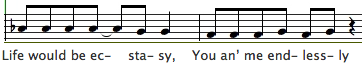
\includegraphics{page2image5568.png}}
\end{center}
\label{page2image5568.png}
\end{figure}



In this musical phrase, the emphasis always goes on the first part of a beat (for the purposes of this example, a ``beat'' is defined as a quarter note).
In this case, the first measure is emphasized for the notes that correspond to the lyrics, ``Life'', ``be'', ``ec-''(as in ec-sta- sy) and ``sy''(again, as in ec-sta-sy) (This is a vast oversimplification, but it works for now). So, the lyrics would be emphasized as such:
\begin{figure}
\begin{center}
\resizebox{1\linewidth}{!}{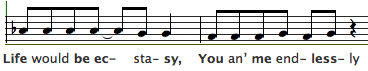
\includegraphics{page2image44544.png}}
\end{center}
\label{page2image44544.png}
\end{figure}

    . \\
Or, more simply:
Life would be ec-sta-sy
This musical emphasis matches the spoken emphasis of the phrase, so it is intelligible as a lyric. (Though ecstasy's first syllable doesn't start on the first part of beat three, it is still on the first part of beat three, and therefore still emphasized. Alternatively, since the first part of beat two didn't have a hard stop to it, the emphasis could have rolled over to the second part, ``ec'', which does have a hard stop.)
In contrast, take the second measure: the syllables ``You'', ``me'', and ``less'' are emphasized in the music. This leads to conflicting musical and spoken phrasing:
Musical Phrasing: You and me endlessly 
Spoken Phrasing: You and me endlessly
The singer is now singing the phrase, syllable by syllable, which they think of as syllable-note combinations:
YOU and ME end LESS lee
The singer, for his part, is doing what many singers are taught to do, to make it easier to sustain the singing of words that end with unsingable consonants: the unsingable consonant is displaced onto the front of the next word. In this case, the consonant ``d'' is not singable, so he displaces it onto the next syllable, when he can: ``and ME'' becomes ``an dME'', and ``end LESS'' becomes ``en dLESS''. So, the singer can effectively think of the sung phrase as:
YOU an dME en dLESS lee


This doesn't cause confusion for listeners, because they're used to hearing it. This does mean, however, that lyric placement does not provide an accurate barometer to a listener of where a word actually ends.
In addition, the singer is singing fudging his vowels, like singers are taught to do, so ``and'' and ``end'' sound almost indistinguishable. So, really, what listeners are hearing is this:
YOU en dME en dLESS lee


Now, the listener's brain has to take this syllabic gobbledy- gook, and parse it into something useful. They've currently got this mess to deal with (represented in SAMPA syllables):
ju En dmi En dl@s li

They parse the first part just fine, because the emphases
you and me En dl@s li
But no one says endLESSly. People say ENDlessly. So, the listeners don't recognize it. They have to work with what they have. They already turned one ``En d'' into an ``and'', so they do it again:
you and me and l@s li
Now, they're just left with LESS lee. And that fits Leslie, a proper noun that fits in context and in emphasis placement. So, the final heard lyric is:
you and me and Les- lie
The misunderstanding can be traced back to improper emphasis placement. The songwriter probably didn't even think of that, and now he's stuck: a one-hit-wonder with a misunderstood song. We bet that in interview after interview, someone asks him who Leslie is. It's probably very frustrating --- especially since he could have just moved the word an eight note later, and it would have been understood perfectly.
That's the sort of situation this program is going to help avoid.
III. FUTURE WORK
We plan to continue developing and refining the methods through which Melody Matcher makes its determinations. Eventually, we plan to use this as an underlying framework for an interactive virtual environment where your surroundings are affected and created via musical and lyrical input. This should be completed in March 2012, with incremental updates discussed on www.melodymatcher.com.
IV. CONCLUSION
In this paper, we have discussed at a high level parts of the music-lingustic approach that Melody Matcher takes to measure the intelligibility of lyrics. We covered some of the major reasons that lyrics get misheard, along with a few examples. Melody Matcher's specific implementation details, while fully specified elsewhere, were outside the scope of this abstract, and we hope to cover them in a later paper.


%
% Back Matter
%

\backmatter
%\appendixpage

%	Bibliography
\bibliographystyle{\mybibliostyle}
\bibliocommand

%	Glossary
\printglossary


%	Index
\printindex

\end{document}
